%%%%%%%%%%%%%%%%%%%%%%%%%%%%%%%%%%%%%%%%%
% wasmCat — Bachelor Thesis Defense Slides
% Structure: Method (Phương pháp) -> Process (Quá trình) -> Result (Kết quả)
% Based on the LaTeXTemplates.com Beamer template (CC BY-NC-SA 4.0)
%%%%%%%%%%%%%%%%%%%%%%%%%%%%%%%%%%%%%%%%%

\documentclass[11pt, aspectratio=169]{beamer}

\graphicspath{{images/}{./}}

\usepackage{booktabs}
\usepackage{listings}

%----------------------------------------------------------------------------------------
%	THEME
%----------------------------------------------------------------------------------------

\usetheme{Madrid}
\usefonttheme{default}
\usepackage[utf8]{inputenc}
\usepackage[T1,T5]{fontenc} % T5 enables Vietnamese diacritics with pdflatex
\usepackage{palatino}
\usepackage[default]{opensans}
\useinnertheme{circles}

\setbeamertemplate{navigation symbols}{}

% Compact code style for showing input/output data structures
\lstset{
	basicstyle=\ttfamily\scriptsize,
	keywordstyle=\color{blue!55!black}\bfseries,
	commentstyle=\color{green!40!black}\itshape,
	stringstyle=\color{orange!80!black},
	morekeywords={string,float64,uint32,uint64,struct,int,bool,time.Time},
	columns=fullflexible,
	keepspaces=true,
	showstringspaces=false,
	aboveskip=3pt, belowskip=1pt,
}

%----------------------------------------------------------------------------------------
%	PRESENTATION INFORMATION
%----------------------------------------------------------------------------------------

\title[wasmCat]{Geo-Aware WebAssembly (WASM)\\Serverless Orchestrator}
% \subtitle{Bachelor Thesis Defense}
\author[Cao Trần Khánh Linh]{Cao Trần Khánh Linh - 23BI14252}
\institute[USTH]{University of Science and Technology of Hanoi \\ Department of Information and Communication Technology \\ \smallskip \textit{External Supervisor: Eng. Trần Tuấn Anh \quad Internal Supervisor: Assoc. Prof. Trần Giang Sơn}}

\date{July 13, 2026}

\begin{document}

%========================================================================
% 1. TITLE
%========================================================================
\begin{frame}
	\titlepage
\end{frame}

%========================================================================
% 2. OUTLINE
%========================================================================
\begin{frame}
	\frametitle{Outline}
	\tableofcontents
\end{frame}

%========================================================================
\section{Introduction}
%========================================================================

%3. Context
\begin{frame}
	\frametitle{Context}
	\begin{columns}[t]
		\begin{column}{0.5\textwidth}
			\textbf{Edge computing}
			\begin{itemize}
				\item Compute close to the data / user
				\item Latency-sensitive workloads
				\item \emph{Where} matters, not only \emph{how much}
			\end{itemize}
		\end{column}
		\begin{column}{0.5\textwidth}
			\textbf{Serverless}
			\begin{itemize}
				\item Submit \emph{prebuilt functions}, not servers
				\item Platform picks node, runs, returns
				\item Developers never pick worker manually
			\end{itemize}
		\end{column}
	\end{columns}
	\bigskip
	\textbf{wasmCat}: Native Go master-worker orchestrator running WebAssembly functions on geo-distributed edge workers with \textbf{no container runtime}.
\end{frame}

%4. Why Wasm not containers
\begin{frame}
	\frametitle{Why WebAssembly?}
	\begin{columns}[t]
		\begin{column}{0.5\textwidth}
			\textbf{Container overhead}
			\begin{itemize}
				\item Image pull + layer unpack
				\item Namespace / cgroup setup
				\item Heavy control plane
				\item Scheduling ignores geography
			\end{itemize}
		\end{column}
		\begin{column}{0.5\textwidth}
			\textbf{WebAssembly + wazero}
			\begin{itemize}
				\item One \texttt{.wasm} file
				\item Sandbox: linear memory only
				\item Compile once, instantiate per request 
				\item Run on any worker with Go runtime
			\end{itemize}
		\end{column}
	\end{columns}
	\bigskip
	\textbf{=>} Edge functions need fast startup + minimal dependencies + \textbf{location-aware} placement.
\end{frame}

%5. Contributions
\begin{frame}
	\frametitle{Contributions}
	\begin{enumerate}
		\item Go-native master-worker orchestrator
		\item Capacity-aware \textbf{geo-routing} scheduling with Haversine formula 
		\item Embedded \textbf{wazero}: digest-aware cache, strict limits
		\item \textbf{Security}: mTLS, certificate-bound identity, digest verification
		\item \textbf{Reliability}: durable SQLite jobs, idempotency
		\item \textbf{Tooling}: CLI, web dashboard
	\end{enumerate}
\end{frame}

%========================================================================
\section{Architectural Design}
%========================================================================

%6. Architecture
\begin{frame}
	\frametitle{System Architecture}
	\begin{figure}
		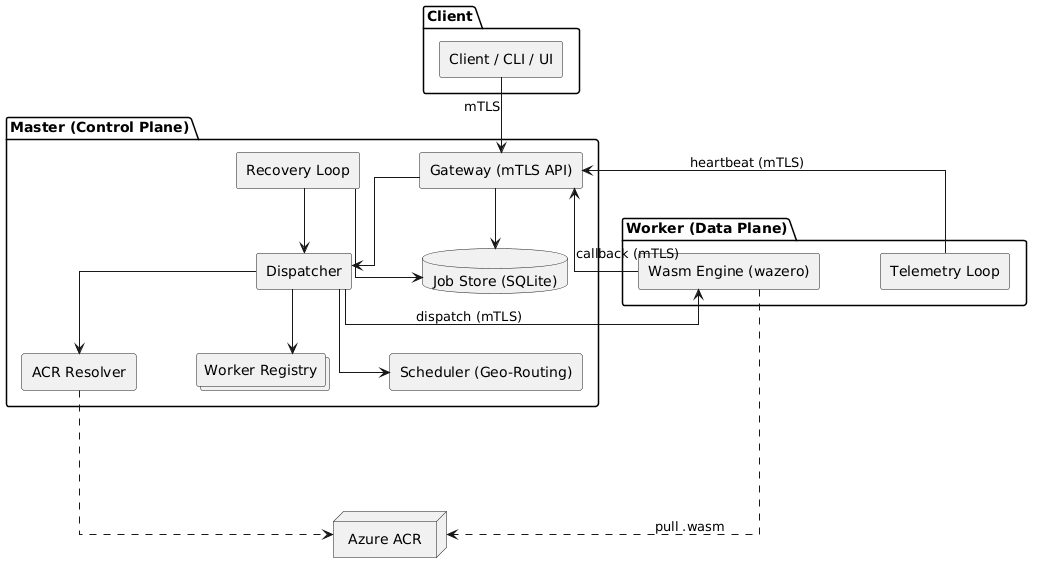
\includegraphics[height=0.72\textheight]{architecture_diagram.png}
		% \caption{Master and workers over mTLS: gateway, registry, geo-scheduler, dispatcher, ACR resolver, SQLite jobs.}
	\end{figure}
\end{frame}

%7. INPUT / OUTPUT data model  (KEY)
\begin{frame}[fragile]
	\frametitle{Data Model: Input $\rightarrow$ Output}
	\begin{columns}[t]
		\begin{column}{0.5\textwidth}
			\textbf{INPUT (\texttt{ExecutionRequest})}
\begin{lstlisting}
struct {
  RequestID          string
  ModuleName         string
  Payload            string
  ModuleRegistryURL  string
  ModuleDigest       string
  UserLat            float64
  UserLon            float64
}
\end{lstlisting}
		\end{column}
		\begin{column}{0.5\textwidth}
			\textbf{OUTPUT (\texttt{ExecutionResponse})}
\begin{lstlisting}
struct {
  RequestID        string
  Result           string  
  ExecutionTimeMs  float64
  ExecutedOnNodeID string  
  Error            string  
}
\end{lstlisting}
		\end{column}
	\end{columns}
	\bigskip
	\begin{center}
		\small \texttt{POST /api/v1/execute} $\;\Rightarrow\;$ JSON in $\;\rightarrow\;$ JSON out (same request\_id)
	\end{center}
\end{frame}

%8. Worker model  (KEY)
\begin{frame}[fragile]
	\frametitle{Worker Model \& Registry}
	\begin{columns}[t]
		\begin{column}{0.52\textwidth}
			\textbf{One worker = one \texttt{WorkerNode}}
\begin{lstlisting}
struct {
  ID        string
  IPAddress string
  Latitude  float64
  Longitude float64
  CPUFree   float64   
  RAMFreeMB float64
  LastSeen  time.Time
  State     string    
}
\end{lstlisting}
		\end{column}
		\begin{column}{0.46\textwidth}
			\textbf{Registry = \texttt{map[ID]WorkerNode}}
			\begin{itemize}
				\item In memory, behind a \texttt{sync.RWMutex}: many reads, rare writes
				\item \textbf{Heartbeat} every 5\,s updates only CPU / RAM
				\item Coordinates set once, at registration
				\item Background loop evicts workers that go silent
			\end{itemize}
			\medskip
			% {\small\itshape In memory on purpose: liveness is real-time state, not durable data --- durability is for jobs.}
		\end{column}
	\end{columns}
\end{frame}

%9. Scheduling method
\begin{frame}
	\frametitle{Scheduling}
	\begin{columns}[c]
		\begin{column}{0.5\textwidth}
			\textbf{Two stages}
			\begin{enumerate}
				\item \textbf{Filter}: drop \texttt{draining}, then below CPU/RAM thresholds
				\item \textbf{Score}: nearest by great-circle distance
			\end{enumerate}
			\smallskip
			\emph{Input}: \texttt{user\_lat/lon} + workers\\
			\emph{Output}: one \texttt{WorkerNode}
		\end{column}
		\begin{column}{0.48\textwidth}
			\textbf{Haversine} ($R=6371$\,km)
			\begin{equation*}
				a = \sin^2\!\tfrac{\Delta\mathrm{lat}}{2} + \cos\mathrm{lat}_1\cos\mathrm{lat}_2\sin^2\!\tfrac{\Delta\mathrm{lon}}{2}
			\end{equation*}
			\begin{equation*}
				d = R\cdot 2\,\mathrm{atan2}(\sqrt{a},\sqrt{1-a})
			\end{equation*}
		\end{column}
	\end{columns}
	\bigskip

		{\small\itshape Shorter distance usually lowers latency, but the network path and congestion also matter.}

\end{frame}

% 10. Execution Modes
\begin{frame}[fragile]
	\frametitle{Execution Modes}
	Two ways to pass data in and read the result out:
	\medskip
	\begin{columns}[t]
		\begin{column}{0.52\textwidth}
			\textbf{wasmCat ABI}: 
\begin{lstlisting}
// module exports: run
run(ptr, len) -> packed uint64
// host writes input to memory,
// calls run, reads output back
\end{lstlisting}
			{\small Minimal \& fast, but module must be built for it.}
		\end{column}
		\begin{column}{0.46\textwidth}
			\textbf{WASI}: 
\begin{lstlisting}
// module exports: _start
stdin  <- payload
stdout -> result
\end{lstlisting}
			{\small Any Rust / Go / C build runs unchanged.}
		\end{column}
	\end{columns}
	\medskip

	\textbf{Worker auto-picks} from the module's exports: \texttt{run} $\to$ wasmCat ABI, \texttt{\_start} $\to$ WASI.\\
	Both: compiled once (digest cache), fresh instance per request.
\end{frame}

% 11. Security method
\begin{frame}
	\frametitle{Security Model}
	\begin{enumerate}
		\item \textbf{mTLS}: Verified client cert before any handler
		\item \textbf{Certificate-bound identity}: Claimed worker ID must equal cert CN / DNS SAN $\Rightarrow$ no impersonation
		\item \textbf{Module integrity}: Verified SHA-256 hash before compile
		\item \textbf{Scoped credentials}: ACR token: repository-scoped, pull-only, short-lived
	\end{enumerate}
	% \bigskip
	% \begin{block}{Boundary preserved}
	% 	Dashboard never talks to the master from the browser, but a local backend reuses the same mTLS client. Private keys never leave the host.
	% \end{block}
\end{frame}

%========================================================================
\section{Execution Lifecycle}
%========================================================================

% 12. Synchronous execution process (I/O concrete)
\begin{frame}[fragile]
	\frametitle{Synchronous Execution: Input $\rightarrow$ Process $\rightarrow$ Output}
	\begin{columns}[t]
		\begin{column}{0.46\textwidth}
			\textbf{Pipeline}
			\begin{enumerate}
				\item Validate + idempotency (\texttt{request\_id})
				\item Resolve ACR (if needed)
				\item Scheduler $\rightarrow$ nearest worker
				\item \texttt{/invoke} over mTLS
				\item Worker: fetch/compile, run, read output
			\end{enumerate}
		\end{column}
		\begin{column}{0.54\textwidth}
			\textbf{Input}
\begin{lstlisting}
{ "request_id":"req_demo_001",
  "module_name":"jsonfmt",
  "payload":"{\"b\":2,\"a\":1}",
  "user_lat":1.29, "user_lon":103.85 }
\end{lstlisting}
			\textbf{Output}
\begin{lstlisting}
{ "request_id":"req_demo_001",
  "result":"{\n \"a\":1,\n \"b\":2\n}",
  "execution_time_ms":2.932,
  "executed_on_node_id":"worker-vn-01" }
\end{lstlisting}
		\end{column}
	\end{columns}
\end{frame}

% 13. Durable job process + state machine
\begin{frame}
	\frametitle{Durable Job Process \& State Machine}
	\begin{columns}[c]
		\begin{column}{0.5\textwidth}
			\begin{itemize}
				\item \texttt{POST /api/v1/jobs} $\rightarrow$ \texttt{202}, persisted in \textbf{SQLite}
				\item Recovery loop leases + dispatches queued jobs
				\item \textbf{Idempotency}: same fingerprint $\rightarrow$ replay; different $\rightarrow$ \texttt{409}
			\end{itemize}
			\begin{alertblock}{\texttt{ambiguous}}
				Lease expired, execution unconfirmed $\Rightarrow$ mark \texttt{ambiguous}, never retry blindly. 
			\end{alertblock}
		\end{column}
		\begin{column}{0.48\textwidth}
			\begin{figure}
				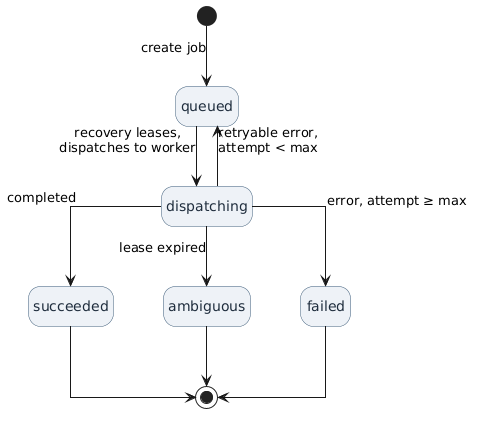
\includegraphics[width=\linewidth]{state_machine_diagram.png}
				\caption{Job lifecycle}
			\end{figure}
		\end{column}
	\end{columns}
\end{frame}

% 14. ACR JIT provisioning process
\begin{frame}
	\frametitle{JIT Module Provisioning from Azure ACR}
	\begin{enumerate}
		\item Detect *.azurecr.io reference
		\item Master: DefaultAzureCredential $\rightarrow$ token repository:<name>:pull
		\item Fetch OCI manifest $\rightarrow$ pick application/wasm layer $\rightarrow$ blob URL
		\item Forward \{blob URL + bearer + digest\} to worker $\rightarrow$ download \& compile
	\end{enumerate}
	\bigskip
	\begin{block}{Property}
		Workers hold \textbf{no} Azure credentials, only a per-request, repository-scoped, pull-only token. Modules published as OCI artifacts with \textbf{ORAS}.
	\end{block}
\end{frame}

%========================================================================
\section{Results}
%========================================================================

% 15. Result 1: geo-routing
\begin{frame}
	\frametitle{Result 1: Geo-routing}
	\begin{table}
		\centering
		\begin{tabular}{|l|l|l|}
			\hline
			\textbf{Client coords} & \textbf{Location} & \textbf{Selected worker}\\
			\hline
			1.29, 103.85 & Singapore & worker-vn-01 (SEA) \\
			\hline
			47.67, $-$122.12 & Seattle & worker-west-us-01 (US) \\
			\hline
		\end{tabular}
		\caption{Same request, different coordinates $\rightarrow$ nearest eligible worker.}
	\end{table}
	\begin{itemize}
		\item \textbf{Draining}: drained worker excluded; traffic shifts to the ready one
		\item \textbf{mTLS}: plain \texttt{curl} (no client cert) rejected at transport layer
	\end{itemize}
\end{frame}

% 16. Result 2: latency
\begin{frame}
	\frametitle{Result 2: Latency}
	\begin{table}
		\centering
		\begin{tabular}{|l|r|r|}
			\hline
			\textbf{Module source} & \textbf{Cold (ms)} & \textbf{Warm (ms)}\\
			\hline
			Direct HTTP URL & 2135.559 & 7.529 \\
			\hline
			Azure ACR (OCI) & 2372.821 & 2.932 \\
			\hline
		\end{tabular}
		\caption{Worker \texttt{execution\_time\_ms} by source and cache state.}
	\end{table}
	\begin{itemize}
		\item Cold $\approx$ download + wazero compile: paid \textbf{once} per version per worker
		\item Warm $\approx$ fresh instance from cache: a few ms
		\item No image pull / namespace setup on any request
	\end{itemize}
\end{frame}

% 17. Limitations
\begin{frame}
	\frametitle{Limitations}
	\begin{enumerate}
		\item \textbf{Single master}: local SQLite recovery, \emph{not} HA
		\item \textbf{In-memory registry}: membership rebuilt from heartbeats after restart
		\item \textbf{Haversine $\neq$ RTT}: no congestion / cache-locality awareness
		\item \textbf{Coarse isolation}: host-level CPU/RAM, no per-invocation cgroup / fuel
		\item \textbf{Workload}: stateless functions only (no sockets / FS beyond \texttt{wasip1})
	\end{enumerate}
\end{frame}

%========================================================================
\section{Conclusion}
%========================================================================

% 18. Conclusion
\begin{frame}
	\frametitle{Conclusion \& Future Work}
	\begin{block}{Demonstrated}
		A compact native Go system: capacity- \& location-aware scheduling, JIT ACR provisioning, mTLS, durable idempotent jobs on a two-region Azure VM deployment.
	\end{block}
	\bigskip
	\textbf{Future work}
	\begin{itemize}
		\item High Availability control plane: leader election + external job store
		\item Smarter scheduling: RTT, queue depth, cache locality
		\item Stronger isolation: fuel metering, cgroups, admission control
		\item Wider model: HTTP-handler ABI, WASI-HTTP, component model
	\end{itemize}
\end{frame}

% 19. Thank you
\begin{frame}[plain]
	\begin{center}
		{\Huge Thank you for listening}\\[1.2em]
	\end{center}
\end{frame}

\end{document}